% =========================================================================
% Tentativo 18: il punteggio esatto NewsGuard (0-100), solo regressione. Che cosa si fa, passo per passo:
% dataset, split, condizioni dei dati, modelli, addestramento, valutazione. I risultati sono nel notebook
% Code/WebScience2027/Tentativi/18_PunteggioEsatto/04_confronto.ipynb.
% Figure: figure/genera_figure.py (legge Dataset/).   Build: tectonic punteggio_esatto.tex
% =========================================================================
\documentclass[aspectratio=169]{beamer}
\usetheme{Madrid}
\usecolortheme{whale}
\usepackage[T1]{fontenc}
\usepackage{graphicx}
\usepackage{booktabs}
\usepackage{array}
\usepackage{xcolor}
\graphicspath{{./figure/}{./}}

\beamertemplatenavigationsymbolsempty
\newcommand{\hl}[1]{\textbf{#1}}
\newcommand{\divider}[2]{%
  \begin{frame}[plain]
    \vfill
    \begin{center}
      {\color{dividerblue}\Huge\textbf{#1}}\\[0.8em]
      {\large #2}
    \end{center}
    \vfill
  \end{frame}}
\definecolor{dividerblue}{RGB}{28,42,92}

\title[Il punteggio esatto]{Il punteggio esatto}
\subtitle{Tentativo 18: prevedere il punteggio NewsGuard (0--100) di una testata dai suoi articoli, senza classi}
\author[John Bianchi]{John Bianchi}
\institute[]{IMT Lucca \& IIT-CNR Pisa}
\date{}

\begin{document}

\begin{frame}
  \titlepage
\end{frame}

\begin{frame}{La domanda e i dubbi da togliere}
  \vfill
  \hl{La domanda}: dai soli articoli di una testata mai vista, quanto bene si prevede il suo \hl{punteggio NewsGuard}, come
  numero da 0 a 100? Niente classi n\'e livelli, in nessun punto.\\[1em]
  \hl{I dubbi sulla regressione fatta finora} (tentativo 16):
  \begin{enumerate}
    \setlength\itemsep{0.5em}
    \item i fold erano stratificati sui \hl{5 livelli}: il punteggio \hl{dentro} un livello era lasciato al caso;
    \item l'addestramento \`e per articolo e le testate hanno da 10 a 201 articoli: \hl{chi scrive di pi\`u pesa di pi\`u};
    \item la valutazione passava per le classi (quote del training): non si misurava mai \hl{di quanti punti} si sbaglia;
    \item non sapevamo se prevedere il numero serve davvero, rispetto a un classificatore.
  \end{enumerate}
  \vfill
\end{frame}

% ===================================================================================================
\divider{1. I dati}{lo stesso dataset del tentativo 16}

\begin{frame}{Il dataset, passo per passo}
  \vfill
  \small
  \begin{enumerate}
    \setlength\itemsep{0.45em}
    \item Testate con NewsGuard 2026 e un solo argomento, ``notizie o commenti politici''; lo scraping di ottobre 2026.
    \item Il testo di ogni articolo riestratto dalla pagina HTML con trafilatura in modalit\`a precisione.
    \item Solo inglese, \hl{da 100 a 1.500 parole} (ogni articolo entra intero in 2.048 token), pubblicati dal 2025.
    \item Doppioni e quasi doppioni tolti tra tutte le testate (si tiene la copia pi\`u vecchia).
    \item Almeno 10 articoli per testata; \hl{una sola testata per gruppo} di propriet\`a (Owner o Parent Domain di NewsGuard).
    \item A ogni articolo il punteggio della sua testata.
  \end{enumerate}
  \vspace{0.8em}
  \centering
  {\Large \hl{226 testate, 25.524 articoli}}\\[0.3em]
  \raggedright
  Le etichette sono \hl{per testata}: tutti gli articoli di una testata hanno lo stesso punteggio.
  \vfill
\end{frame}

\begin{frame}{Il punteggio e gli articoli}
  \centering
  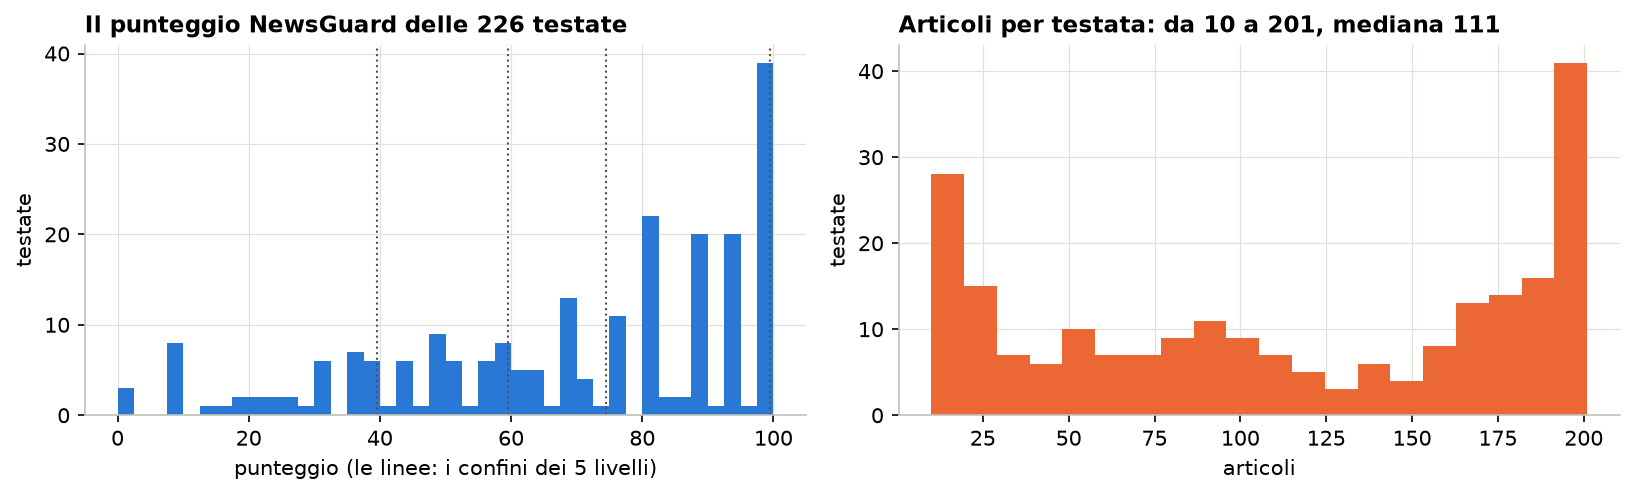
\includegraphics[width=0.97\textwidth]{dataset.png}\\[0.4em]
  \raggedright\small
  \begin{itemize}
    \item Il punteggio \`e la somma dei punti di 9 criteri: solo \hl{45 valori diversi}; 39 testate a 100, 3 a 0; media 68,5.
    \item Gli articoli per testata vanno da 10 a 201: le testate pi\`u prolifiche hanno 20 volte gli articoli delle altre.
  \end{itemize}
\end{frame}

% ===================================================================================================
\divider{2. Gli split}{stratificati sul punteggio, non sui livelli}

\begin{frame}{Come si fa lo split nuovo}
  \centering
  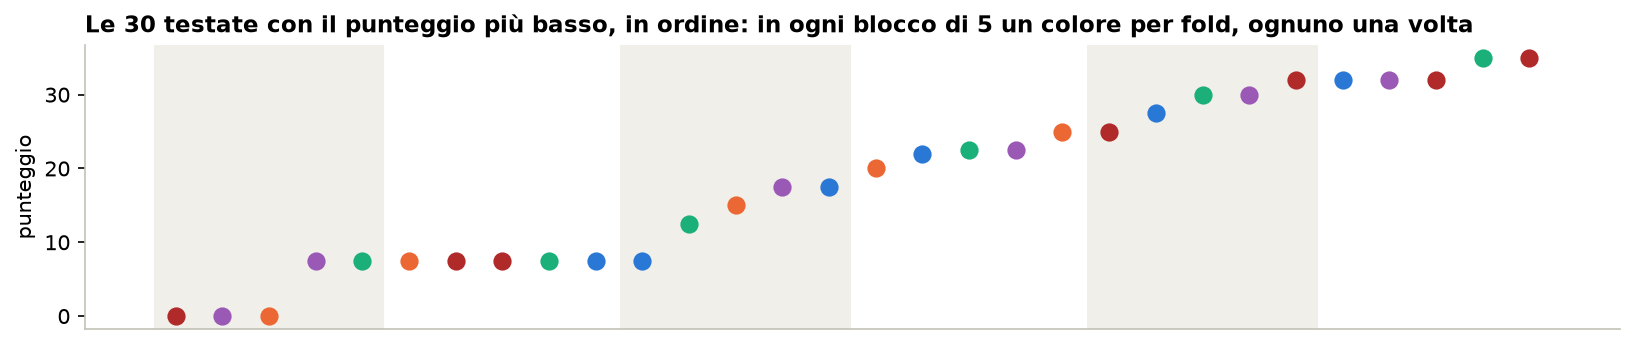
\includegraphics[width=0.97\textwidth]{come_si_fa_lo_split.png}\\[0.4em]
  \raggedright\small
  \begin{enumerate}
    \item Le 226 testate si ordinano per punteggio (a parit\`a di punteggio, in ordine casuale).
    \item A blocchi di 5 consecutive, ogni testata va in un fold diverso (un colore per fold).
    \item Ogni fold riceve cos\`i testate di tutti i punteggi, anche dentro lo stesso livello.
    \item Si ripete con \hl{3 semi diversi}: tre split, per misurare quanto i risultati dipendono dallo split.
  \end{enumerate}
\end{frame}

\begin{frame}{Split vecchi e nuovi}
  \centering
  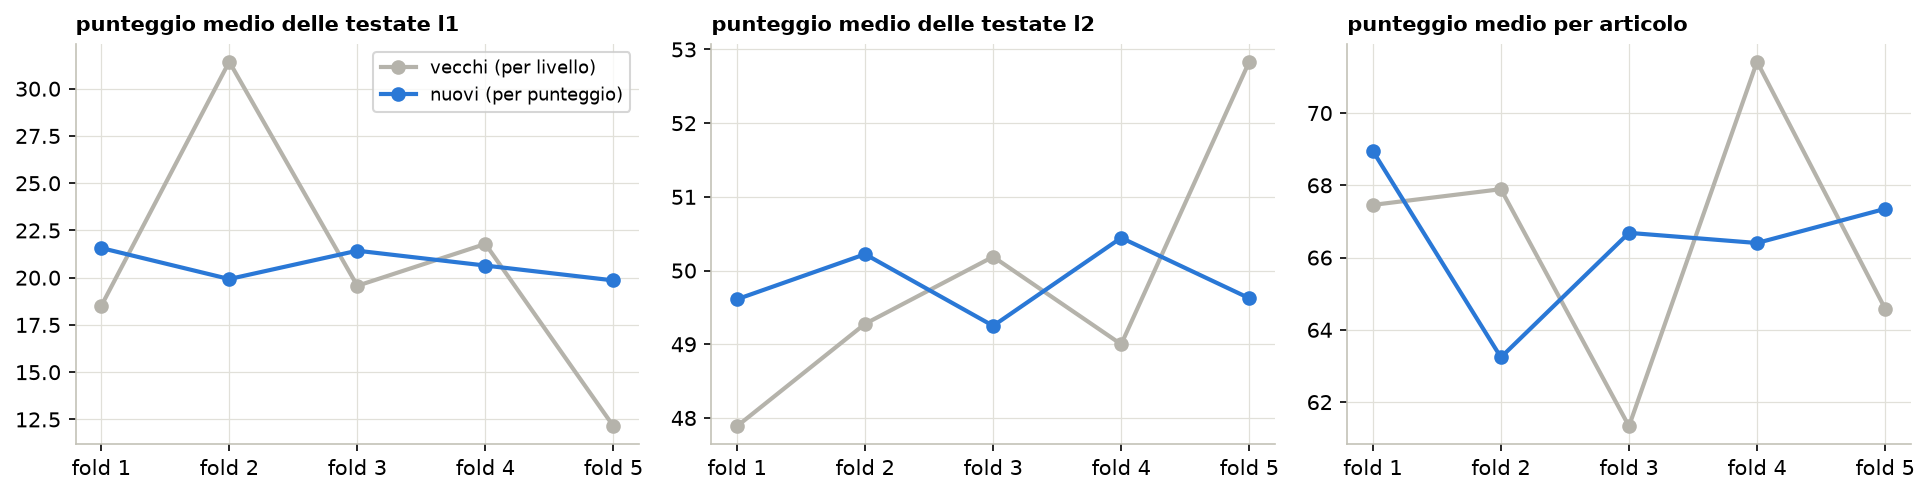
\includegraphics[width=0.97\textwidth]{split_vecchi_nuovi.png}\\[0.4em]
  \raggedright\small
  \begin{itemize}
    \item \hl{Dentro i livelli}: con i vecchi split le testate l1 di un fold avevano in media da 12 a 31 punti; ora da 20 a 22.
    \item \hl{Per articolo} la media cambia ancora tra i fold (da 63 a 69): dipende da quanti articoli hanno le testate di
          ogni fold. Questo lo affrontano le condizioni dei dati.
  \end{itemize}
\end{frame}

% ===================================================================================================
\divider{3. Le condizioni dei dati}{quanto pesa ogni testata in addestramento}

\begin{frame}{Cinque condizioni}
  \centering
  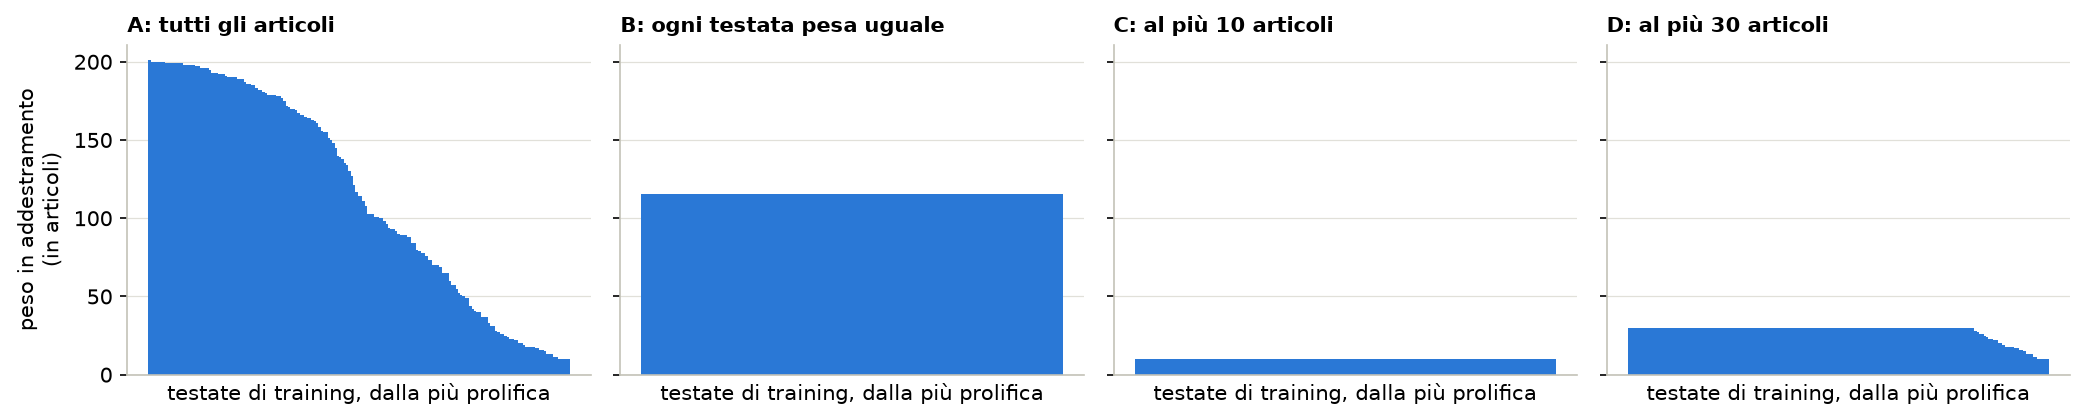
\includegraphics[width=0.97\textwidth]{condizioni.png}\\[0.3em]
  \raggedright\small
  \begin{tabular}{cl}
    \textbf{A} & tutti gli articoli, peso 1: chi scrive di pi\`u pesa di pi\`u (come finora) \\
    \textbf{B} & tutti gli articoli, peso $1/(\text{articoli della testata})$: \hl{ogni testata pesa uguale} \\
    \textbf{C} & al pi\`u \hl{10 articoli} per testata, presi a caso (10 \`e il minimo del dataset) \\
    \textbf{D} & al pi\`u \hl{30 articoli} per testata \\
    \textbf{E} & \hl{un vettore per testata}: la media dei vettori dei suoi articoli; il modello impara sulle testate \\
  \end{tabular}\\[0.4em]
  Cambia solo l'addestramento: \hl{il test sono sempre tutti gli articoli} delle testate di test.
\end{frame}

\begin{frame}{Il peso per testata: il ``learning rate'' giusto}
  \vfill
  \begin{itemize}
    \setlength\itemsep{0.9em}
    \item In un modello lineare (ridge, logistica) il modo corretto di dire ``impara meno da questa testata'' \`e il
          \hl{peso degli esempi}: l'errore di ogni articolo conta in proporzione al suo peso.
    \item Condizione B: ogni articolo pesa $1/n$, dove $n$ sono gli articoli della sua testata. Una testata con 200 articoli
          e una con 10 contribuiscono allo stesso modo.
    \item Nei BERT addestrati si fa la stessa cosa nell'errore quadratico di ogni lotto: $\sum_i w_i (\hat y_i - y_i)^2 / \sum_i w_i$.
    \item C e D ottengono lo stesso effetto in un altro modo, buttando via articoli; E lo porta all'estremo: una sola riga per testata.
  \end{itemize}
  \vfill
\end{frame}

% ===================================================================================================
\divider{4. I modelli}{chi legge il testo e chi prevede il numero}

\begin{frame}{Chi legge il testo}
  \vfill
  \small
  \begin{tabular}{>{\raggedright\arraybackslash}p{0.2\textwidth}>{\raggedright\arraybackslash}p{0.42\textwidth}>{\raggedright\arraybackslash}p{0.27\textwidth}}
    \toprule
    \textbf{Lettore} & \textbf{Come diventa numeri} & \textbf{Si addestra?} \\
    \midrule
    TF-IDF & parole e coppie di parole (100.000), pesate per rarit\`a; vocabolario dai soli testi di training & no (solo il modello sopra) \\
    \addlinespace
    Mistral-Small 24B & LLM da 24 miliardi di parametri, in 4 bit; il vettore \`e la media degli stati interni dei token allo
    strato 27 di 40 (5.120 numeri) & \hl{no}: \`e congelato, un lettore \\
    \addlinespace
    ModernBERT-base & 150 milioni di parametri, articoli interi (2.048 token) & \hl{s\`i}, tutto \\
    \addlinespace
    DeBERTa-v3-base & 184 milioni di parametri, un'architettura diversa; i primi 512 token & \hl{s\`i}, tutto \\
    \bottomrule
  \end{tabular}\\[1em]
  \raggedright
  Sopra TF-IDF e Mistral: \hl{ridge} (regressore) o \hl{logistica} (classificatore). ModernBERT e DeBERTa hanno un neurone in
  uscita che \`e direttamente il punteggio.
  \vfill
\end{frame}

\begin{frame}{Regressore o classificatore? Come si confrontano}
  \vfill
  \begin{itemize}
    \setlength\itemsep{0.8em}
    \item \hl{Regressore}: la ridge impara il punteggio 0--100 e d\`a un numero per articolo.
    \item \hl{Classificatore}: la logistica impara i 5 livelli e d\`a 5 probabilit\`a per articolo. Per confrontarlo sullo
          stesso terreno, le probabilit\`a diventano un punteggio: la media dei punteggi medi di ogni livello nel training,
          pesata con le probabilit\`a.
  \end{itemize}
  \vspace{0.6em}
  \centering\small
  \begin{tabular}{lccccc}
    \toprule
    livello & l1 & l2 & l3 & l4 & l5 \\
    \midrule
    punteggio medio nel training (circa) & 21 & 50 & 67 & 85 & 100 \\
    probabilit\`a date dal classificatore & 0,1 & 0,2 & 0,3 & 0,3 & 0,1 \\
    \bottomrule
  \end{tabular}\\[0.5em]
  punteggio previsto $= 0{,}1\cdot21 + 0{,}2\cdot50 + 0{,}3\cdot67 + 0{,}3\cdot85 + 0{,}1\cdot100 = 67{,}7$\\[0.8em]
  \raggedright
  Se il regressore non fa meglio di questo, prevedere il numero non aggiunge nulla.
  \vfill
\end{frame}

\begin{frame}{Come si addestrano}
  \vfill
  \small
  \begin{itemize}
    \setlength\itemsep{0.7em}
    \item \hl{Ridge}: i pesi minimizzano l'errore quadratico pesato pi\`u una penalit\`a (alpha) sui pesi grandi, che evita di
          imparare a memoria. \hl{Logistica}: come sopra, sulla probabilit\`a del livello giusto (penalit\`a C).
    \item \hl{La penalit\`a si sceglie dentro il training}: le testate di training si dividono in 3 (sul punteggio), si prova
          ogni valore della griglia e si tiene quello con l'errore medio per testata pi\`u basso; poi si riaddestra su tutto il
          training. Il fold di test non entra mai nella scelta.
    \item \hl{ModernBERT e DeBERTa}: tutto il transformer, errore quadratico pesato sul punteggio/100, lotti di 32 articoli,
          learning rate 3e-5, 5 epoche, si tiene l'ultima. Solo sullo split 1 (ogni corsa costa ore): ModernBERT nelle
          condizioni A, B, C; DeBERTa nella B.
    \item \hl{TF-IDF e Mistral}: tutte le combinazioni, \hl{2 modelli $\times$ 2 tipi $\times$ 5 condizioni $\times$ 3 split
          $\times$ 5 fold = 300 addestramenti}.
  \end{itemize}
  \vfill
\end{frame}

% ===================================================================================================
\divider{5. La valutazione}{di quanti punti si sbaglia, per articolo e per testata}

\begin{frame}{Che cosa si confronta}
  \vfill
  \begin{enumerate}
    \setlength\itemsep{0.8em}
    \item Ogni testata \`e nel test di un fold: \hl{il modello non l'ha mai vista}.
    \item \hl{Articolo singolo}: il punteggio previsto per ogni articolo contro il punteggio vero della sua testata.
    \item \hl{Testata}: la media dei punteggi previsti dei suoi articoli (nella condizione E, la previsione sul vettore medio
          della testata) contro il punteggio vero.
    \item \hl{Riferimento}: chi prevede sempre la media delle testate di training (circa 68,5). Sbaglia in media di
          \hl{22,6 punti} (RMSE 27): un modello serve solo se sta sotto.
  \end{enumerate}
  \vfill
\end{frame}

\begin{frame}{Le misure, con un esempio}
  \small
  Quattro testate:\\[0.4em]
  \centering
  \begin{tabular}{lcccc}
    \toprule
    & testata 1 & testata 2 & testata 3 & testata 4 \\
    \midrule
    punteggio vero & 10 & 50 & 80 & 100 \\
    punteggio previsto & 30 & 55 & 70 & 85 \\
    errore & +20 & +5 & $-$10 & $-$15 \\
    \bottomrule
  \end{tabular}\\[0.7em]
  \raggedright
  \begin{tabular}{>{\raggedright\arraybackslash}p{0.15\textwidth}>{\raggedright\arraybackslash}p{0.48\textwidth}>{\raggedright\arraybackslash}p{0.27\textwidth}}
    \hl{MAE} & errore medio assoluto, in punti & (20+5+10+15)/4 = 12,5 \\
    \hl{RMSE} & radice dell'errore quadratico medio: pesa di pi\`u gli errori grandi & $\sqrt{(400+25+100+225)/4}$ = 13,7 \\
    \hl{R$^2$} & quanta variabilit\`a si spiega (0 = come dire la media, 1 = perfetto) & 1 $-$ 750/4.600 = 0,84 \\
    \hl{Spearman} & l'ordine delle testate \`e giusto? & 1: l'ordine \`e perfetto \\
    \hl{Pearson} & il legame \`e lineare? & 0,998 \\
  \end{tabular}\\[0.5em]
  Nell'esempio l'ordine \`e perfetto ma le previsioni sono \hl{schiacciate verso il centro}: la testata da 10 diventa 30,
  quella da 100 diventa 85. Il MAE lo vede, Spearman no: servono tutte e due.
\end{frame}

\begin{frame}{Le analisi del notebook dei risultati}
  \vfill
  \small
  \begin{enumerate}
    \setlength\itemsep{0.6em}
    \item \hl{Il quadro}: MAE e Spearman, per testata e per articolo, di tutte le configurazioni (media dei 3 split, con il
          minimo e il massimo).
    \item \hl{Regressore o classificatore}: le due curve nelle cinque condizioni, per TF-IDF e Mistral.
    \item \hl{Le migliori configurazioni} con gli intervalli al 95\% (bootstrap sulle testate) e il confronto con la media.
    \item \hl{Dove si sbaglia}: l'errore con il segno e l'errore assoluto per fascia del punteggio vero (0--39, 40--59,
          60--74, 75--99, 100), e il grafico previsto contro vero.
    \item \hl{Il DNA in punti}: la testata giudicata dalla media di 1, 3, 5, 9, 15, 25 articoli o di tutti.
    \item \hl{Quanto conta lo split}: lo stesso modello nei tre split.
  \end{enumerate}
  \vfill
\end{frame}

\begin{frame}{Come leggere i risultati: le domande}
  \vfill
  \small
  \begin{tabular}{>{\raggedright\arraybackslash}p{0.43\textwidth}>{\raggedright\arraybackslash}p{0.47\textwidth}}
    \toprule
    \textbf{Domanda} & \textbf{Dove si legge la risposta} \\
    \midrule
    La regressione aggiunge qualcosa alla classificazione? & regressore contro classificatore trasformato in punteggio \\
    \addlinespace
    Il peso delle testate prolifiche falsava l'addestramento? & condizione A contro B, C, D, E \\
    \addlinespace
    Imparare sulle testate invece che sugli articoli aiuta? & condizione E contro le altre \\
    \addlinespace
    Un BERT addestrato fa meglio di un lettore congelato? & ModernBERT e DeBERTa contro Mistral \\
    \addlinespace
    Di quanti punti si sbaglia, e dove? & MAE contro 22,6 della media; errore per fascia \\
    \addlinespace
    Quanti articoli servono per una testata? & la curva del DNA \\
    \addlinespace
    I risultati dipendono dallo split? & lo stesso modello nei 3 split \\
    \bottomrule
  \end{tabular}
  \vfill
\end{frame}

\begin{frame}{Che cosa ci aspettiamo}
  \vfill
  \begin{itemize}
    \setlength\itemsep{0.8em}
    \item Previsioni \hl{schiacciate verso la media}: con l'errore quadratico, un modello incerto si tiene vicino al centro.
          L'errore per fascia lo mostrer\`a (le testate peggiori sovrastimate, le migliori sottostimate).
    \item Il peso per testata (B) dovrebbe aiutare poco ma rendere i risultati pi\`u stabili tra gli split.
    \item Mistral congelato sopra TF-IDF, come nel tentativo 16; ModernBERT addestrato forse vicino a TF-IDF.
    \item Il DNA: l'errore per testata cala con gli articoli letti e si stabilizza dopo qualche decina.
  \end{itemize}
  \vfill
\end{frame}

\begin{frame}{Dove trovare tutto}
  \vfill
  \small
  \begin{itemize}
    \setlength\itemsep{0.6em}
    \item Codice: \texttt{Code/WebScience2027/Tentativi/18\_PunteggioEsatto/}
      \begin{itemize}
        \item \texttt{01\_split}: gli split; \texttt{02\_lineari}: TF-IDF e Mistral (300 addestramenti, CPU);
        \item \texttt{03\_bert}: ModernBERT e DeBERTa (GPU); \texttt{04\_confronto}: \hl{tutti i risultati};
        \item \texttt{punteggio.py}: le funzioni (split, condizioni, modelli, misure).
      \end{itemize}
    \item Sul server: \texttt{\~{}/John/Tentativo18}, due code in parallelo (\texttt{t18\_cpu}, \texttt{t18\_gpu}); dal PC
          \texttt{./stato.sh} per seguire e \texttt{./scarica.sh} per scaricare.
    \item Gli split sono in \texttt{Dataset/tentativi/18\_PunteggioEsatto/split.csv}.
  \end{itemize}
  \vfill
\end{frame}

\end{document}
